\chapter{张量范畴与弦网模型}

\section{范畴论基础}

\emph{范畴论}(Category theory)用以抽象地刻画一些数学结构之间的关系,它主要描述了“对象”之间的作用,即\emph{映射}(Mapping)。拓扑序理论中所研究的,正是带有了某些附加结构的范畴。

一个\emph{范畴} $\mathcal{C}$ 由其中的\emph{对象}(Object)$x\in\mathcal{C}$ 和对象之间的\emph{态射}(Morphism)$f\colon x\to y$ 组成。对象之间的态射满足以下三个条件:
\begin{itemize}
  \item \emph{复合性}(Composition):对于范畴 $\mathcal{C}$ 中的对象 $x$、$y$、$z$,若 $f\colon x\to y$ 和 $g\colon y\to z$ 为态射,则存在复合态射 $g\circ f\colon x\to z$;
  \item \emph{结合律}(Associativity):若 $\mathcal{C}$ 中有态射 $f\colon x\to y$、$g\colon y\to z$、$h\colon z\to w$,则有
    \begin{equation}
      (h\circ g)\circ f = h\circ (g\circ f);
    \end{equation}
  \item \emph{单位元}(Identity):对于 $\forall x\in\mathcal{C}$,都存在恒等态射 $\id_x\colon x\to x$,使得
    \begin{equation}
      f \circ \id_x = \id_x \circ f = f, \quad \forall f\colon x\to y.
    \end{equation}
\end{itemize}
% 态射也可记为 $f\in\Hom_{\mathcal{C}}(x,y)$,其中 $\Hom_{\mathcal{C}}(x,y)$ 称为同态集(Hom-set)。

\emph{函子}(Functor)是范畴之间保结构的映射。具体而言,对于范畴 $\mathcal{C}$、$\mathcal{D}$,函子 $F\colon\mathcal{C}\to\mathcal{D}$ 会将 $\mathcal{C}$ 中的对象 $x$ 映射到 $\mathcal{D}$ 中的对象 $F(x)$,而将 $\mathcal{C}$ 中的态射 $f\colon x\to y$ 映射到 $\mathcal{D}$ 中的态射 $F_f\colon F(x)\to F(y)$,并且保持复合性与单位元的成立,即
\begin{align}
  F_{\id_x} &= \id_{F(x)} \colon F(x) \to F(x), \quad \forall x\in\mathcal{C}, \\
  F_{g\circ f} &= F_g \circ F_f \colon F(x) \to F(z), \quad \forall f\colon x\to y, \, g\colon y\to z.
\end{align}

在函子之上可进一步定义\emph{自然变换}(Natural transformation)。对于两个函子 $F\colon\mathcal{C}\to\mathcal{D}$ 和 $G\colon\mathcal{C}\to\mathcal{D}$,自然变换 $\tau\colon F\Rightarrow G$ 由其分量 $\tau_x$(这是范畴 $\mathcal{D}$ 中的一个态射)定义:
\begin{equation}
  \tau_x\colon F(x)\to G(x), \quad \forall x\in\mathcal{C},
\end{equation}
它满足
\begin{equation}
  \tau_y \circ F_f = G_f \circ \tau_x, \quad \forall f\colon x\to y.
\end{equation}
若 $\tau$ 的每一分量 $\tau_x$ 均可逆(即存在 $\tau_x^{-1}$ 使得 $\tau^{-1}_x\circ\tau_x=\id_{F(x)}$ 且 $\tau_x\circ\tau^{-1}_x = \id_{G(x)}$),则称其为\emph{自然同构}(Natural isomorphism)。如图~\ref{fig:natural-transformation},自然变换可以用交换图来直观地表示。

\begin{figure}[htb]
  \centering
  \parbox[b]{0.35\textwidth}{
    \centering
    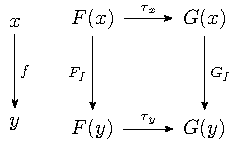
\includegraphics{images/natural-transformation-1.pdf} \\
    (a)
  }
  \parbox[b]{0.55\textwidth}{
    \centering
    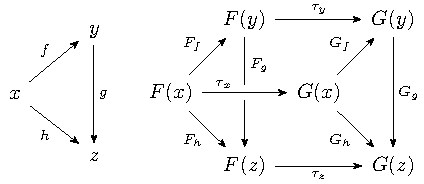
\includegraphics{images/natural-transformation-2.pdf} \\
    (b)
  }
  \caption[自然变换对应的交换图]{自然变换对应的交换图。(a) 此图是“可交换的”,即从 $F(x)$ 到 $G(y)$ 的两条路径等价;(b) 对于结合律的“提升”,图中三棱柱的三个侧面都是可交换的。}
  \label{fig:natural-transformation}
\end{figure}

\section{张量范畴}

\section{拓扑序}

\section{弦网模型}
